\begin{filecontents*}{vibetwin_refs.bib}
@article{zhao2023hybridAE,
  title   = {Novelty Detection and Fault Diagnosis Method for Bearing Faults Based on the Hybrid Deep Autoencoder Network},
  author  = {Zhao, Yuanyuan and Hao, Huijuan and Chen, Yu and Zhang, Yu},
  journal = {Electronics},
  year    = {2023},
  volume  = {12},
  number  = {13},
  pages   = {2826},
  doi     = {10.3390/electronics12132826}
}

@article{hao2023oselm,
  title   = {Incremental Single-Class Fault Detection and Diagnosis Method for Rolling Bearings Based on {OS-ELM}},
  author  = {Hao, Huijuan and others},
  journal = {Electronics},
  year    = {2023},
  volume  = {12},
  number  = {19},
  pages   = {4099},
  doi     = {10.3390/electronics12194099}
}

@article{hendriks2022benchmarking,
  title   = {Towards better benchmarking using the {CWRU} bearing fault dataset},
  author  = {Hendriks, Jacob and Dumond, Patrick and Knox, D. A.},
  journal = {Mechanical Systems and Signal Processing},
  year    = {2022},
  volume  = {169},
  pages   = {108732},
  doi     = {10.1016/j.ymssp.2021.108732}
}

@inproceedings{gal2016dropout,
  title     = {Dropout as a {Bayesian} Approximation: Representing Model Uncertainty in Deep Learning},
  author    = {Gal, Yarin and Ghahramani, Zoubin},
  booktitle = {Proceedings of the 33rd International Conference on Machine Learning ({ICML})},
  year      = {2016},
  note      = {arXiv:1506.02142}
}

@inproceedings{guo2017calibration,
  title     = {On Calibration of Modern Neural Networks},
  author    = {Guo, Chuan and Pleiss, Geoff and Sun, Yu and Weinberger, Kilian Q.},
  booktitle = {Proceedings of the 34th International Conference on Machine Learning ({ICML})},
  year      = {2017},
  note      = {arXiv:1706.04599}
}

@article{zhou2023trustworthy,
  title   = {An uncertainty-informed framework for trustworthy fault diagnosis in safety-critical applications},
  author  = {Zhou, Taotao and Zhang, Laibin and Han, Te and Lopez Droguett, Enrique and Mosleh, Ali and Chan, Felix T. S.},
  journal = {Reliability Engineering \& System Safety},
  year    = {2023},
  doi     = {10.1016/j.ress.2022.108865}
}

@article{du2022igcwt,
  title   = {Integrated Gradient-Based Continuous Wavelet Transform for Bearing Fault Diagnosis},
  author  = {Du, Junfei and Li, Xinyu and Gao, Yiping and Gao, Liang},
  journal = {Sensors},
  year    = {2022},
  volume  = {22},
  number  = {22},
  pages   = {8760},
  doi     = {10.3390/s22228760}
}

@article{ding2023edge,
  title   = {An Edge Intelligent Method for Bearing Fault Diagnosis Based on a Parameter Transplantation Convolutional Neural Network},
  author  = {Ding, Xiang and others},
  journal = {Electronics},
  year    = {2023},
  volume  = {12},
  number  = {8},
  pages   = {1816},
  doi     = {10.3390/electronics12081816}
}

@article{neupane2025review,
  title   = {Data-driven machinery fault diagnosis: A comprehensive review},
  author  = {Neupane, Dhiraj and Bouadjenek, Mohamed Reda and Dazeley, Richard and Aryal, Sunil},
  journal = {Neurocomputing},
  year    = {2025},
  pages   = {129588},
  doi     = {10.1016/j.neucom.2025.129588}
}

@article{lu2025pkeca,
  title   = {Prior knowledge embedding convolutional autoencoder: A single-source domain generalized fault diagnosis framework under small samples},
  author  = {Lu, Feiyu and Tong, Qingbin and Jiang, Xuedong and Du, Xin and Xu, Jianjun and Huo, Jingyi},
  journal = {Computers in Industry},
  year    = {2025},
  volume  = {164},
  pages   = {104169},
  doi     = {10.1016/j.compind.2024.104169}
}

@article{wang2023digitaltwin,
  title   = {Online bearing fault diagnosis using numerical simulation models and machine learning classifications},
  author  = {Wang, Hui and Zheng, Junkang and Xiang, Jiawei},
  journal = {Reliability Engineering \& System Safety},
  year    = {2023},
  volume  = {234},
  pages   = {109142},
  doi     = {10.1016/j.ress.2023.109142}
}
\end{filecontents*}

\documentclass[conference]{IEEEtran}
\usepackage{cite}
\usepackage{graphicx}
\usepackage{url}
\usepackage{amsmath}
\usepackage{amsfonts}
\usepackage{amssymb}
\usepackage{booktabs}

\begin{document}

\title{VibeTwin: An Explainable Generative Digital Twin for Bearing Fault Detection}

\author{\IEEEauthorblockN{Kazi Fardin Islam}
\IEEEauthorblockA{Department of Information and Communication Engineering\\
University of Rajshahi\\
Rajshahi, Bangladesh\\
fardinislamsadnan@gmail.com}}

\maketitle

\begin{abstract}
Early bearing faults are difficult to separate from normal vibration variability because machine signals are noisy, nonstationary, and sensitive to load changes. Many monitoring pipelines still rely on brittle thresholds or closed-set classifiers that can overstate confidence and transfer poorly across operating conditions. This paper presents VibeTwin, a lightweight generative digital twin for bearing vibration monitoring built around a compact 1D-CNN autoencoder trained only on healthy signal windows, with a variational autoencoder retained as a comparison baseline. Faults are detected through reconstruction-based anomaly scoring relative to the learned healthy manifold. To make alerts more reliable, the framework augments reconstruction scores with uncertainty estimates from stochastic inference and calibrated thresholds. It also explains suspicious windows through counterfactual healthy reconstruction and frequency-aware residual analysis that highlights FFT and PSD band changes. Validation is centered on healthy-only training on CWRU, followed by external robustness checks on Paderborn, with XJTU-SY reserved as an optional degradation-oriented extension. In addition to anomaly detection quality, the evaluation plan targets false-alarm behavior, robustness under noise and load shift, explanation usefulness, and edge feasibility through model size and CPU latency.
\end{abstract}

\begin{IEEEkeywords}
bearing fault detection, anomaly detection, autoencoder, explainable AI, uncertainty estimation, edge AI
\end{IEEEkeywords}

\section{Introduction}

Rolling bearings are critical components in rotating machinery, and even small defects can develop into efficiency loss, unplanned downtime, or secondary mechanical damage if they are not detected early. In practice, however, early fault detection remains difficult because vibration signals are noisy, nonstationary, and sensitive to operating conditions such as load and speed. These properties make simple threshold-based monitoring unreliable, while closed-set supervised classifiers often assume access to representative fault labels that may be incomplete in real deployments. For this reason, healthy-only and one-class monitoring strategies have become increasingly attractive for bearing diagnosis, especially when the goal is to detect deviations from normal behavior rather than assign a fixed fault class \cite{zhao2023hybridAE,hao2023oselm}.

A second challenge is that benchmark results can look stronger than real deployment behavior. Prior analysis of the CWRU dataset has shown that naive window-level partitioning, overlap leakage, and recording-specific artifacts may overstate generalization if train and test samples are not carefully separated \cite{hendriks2022benchmarking}. This is particularly relevant for reconstruction-based monitoring, where a model may rank faults well while still transferring poorly across operating conditions. In such settings, raw anomaly scores alone are not enough; threshold calibration becomes important because strong ranking performance does not automatically translate into stable alarm behavior under shift \cite{guo2017calibration}.

This paper presents \emph{VibeTwin}, a healthy-only generative monitoring framework for bearing vibration analysis built around a residual-dilated 1D convolutional autoencoder (ResDilatedAE). Instead of treating bearing monitoring purely as closed-set classification, VibeTwin learns a reconstruction-based reference of healthy behavior and flags deviations through calibrated anomaly scores. The framework also supports qualitative interpretation through healthy reconstruction, residual waveform inspection, and FFT-based comparisons, while keeping deployment practicality in view through model-size and CPU-latency measurements. Empirically, the study uses two complementary evaluation settings: a leakage-safe leave-one-load-out protocol on CWRU for load-shift analysis, and Paderborn for cross-benchmark robustness and deployment-focused validation. The resulting picture is deliberately balanced: stronger generative reconstruction and threshold calibration improve practical healthy-only monitoring, but robust threshold transfer under operating-condition shift remains an open challenge.

\section{Literature Review}

Recent reviews show that machinery fault diagnosis is moving beyond closed-set classification toward settings that better reflect deployment reality, including novelty detection, condition variation, and limited fault labels \cite{neupane2025review}. Within bearing monitoring, healthy-only and one-class methods are especially attractive because normal data are often abundant while complete coverage of all defect types and severities is rarely available. Reconstruction-based autoencoders therefore remain relevant: hybrid deep autoencoder novelty detection has been evaluated on both CWRU and Paderborn \cite{zhao2023hybridAE}, while incremental one-class baselines such as OS-ELM continue to provide useful references for judging whether gains come from representation learning or from threshold choice alone \cite{hao2023oselm}.

A second theme in the literature is that benchmark protocol matters as much as architecture. Reanalysis of CWRU has shown that weak partitioning, overlap leakage, and recording-specific artifacts can inflate apparent generalization \cite{hendriks2022benchmarking}. More recent work on domain-aware and domain-generalized diagnosis reflects the same concern: models are increasingly expected to remain useful under changing working conditions rather than only within convenient random splits. In particular, Lu \emph{et al.} proposed a prior-knowledge-embedded convolutional autoencoder for single-source domain generalization under small samples, highlighting the importance of robustness-oriented feature learning when operating conditions shift \cite{lu2025pkeca}. These findings motivate leakage-safe and condition-aware evaluation protocols for any healthy-only reconstruction model.

Reliability of alarms is another recurring concern. Neural outputs can be miscalibrated even when ranking performance is strong \cite{guo2017calibration}, and MC dropout remains a lightweight way to approximate predictive uncertainty without requiring a fully Bayesian model \cite{gal2016dropout}. In safety-critical diagnosis, uncertainty has therefore been studied as a tool for trustworthy decision support rather than raw confidence reporting \cite{zhou2023trustworthy}. At a broader system level, digital-twin-inspired diagnosis research has also emphasized that monitoring frameworks should remain informative under untrained working conditions and support operational decision making, not only maximize benchmark accuracy \cite{wang2023digitaltwin}. For VibeTwin, this makes calibration and cautious alarm design as important as anomaly scoring itself.

Finally, interpretability and deployability remain practical constraints for real monitoring systems. Frequency-aware explanation methods can make vibration-based decisions easier to inspect by linking model behavior to changes in diagnostically meaningful spectral content \cite{du2022igcwt}. In parallel, edge-oriented diagnosis studies continue to emphasize compact architectures, runtime efficiency, and deployment feasibility rather than accuracy alone \cite{ding2023edge}. Compared with this literature, VibeTwin focuses on a narrower but practically useful gap: a healthy-only generative model evaluated under leakage-safe CWRU load shift and on Paderborn, combined with calibrated thresholds, qualitative reconstruction-plus-FFT explanations, and CPU deployment profiling in one unified study.

\section{Methodology}

VibeTwin is designed as a healthy-only monitoring framework for bearing vibration analysis. Instead of learning a closed-set classifier over predefined fault categories, it learns a compact reconstruction model of normal operating behavior and treats persistent reconstruction mismatch as evidence of abnormality. The final pipeline has four stages: vibration preprocessing and windowing, healthy-only training of a residual-dilated autoencoder, reconstruction-based anomaly scoring with validation-based threshold calibration, and qualitative explanation through healthy reconstruction, residual waveform inspection, and FFT-magnitude analysis.

\subsection{Healthy-Only Monitoring Formulation}

Let $x \in \mathbb{R}^{L}$ denote a fixed-length vibration window, where $L=2048$ in the present study. During training, VibeTwin uses only healthy windows to learn a mapping
\begin{equation}
\hat{x} = f_{\theta}(x),
\end{equation}
where $f_{\theta}(\cdot)$ is the reconstruction model and $\hat{x}$ is the corresponding healthy reconstruction. The core assumption is that a model trained only on normal behavior should reconstruct healthy patterns well, while damaged or shifted patterns should produce larger residual mismatch.

This formulation is attractive for practical condition monitoring because healthy data are usually easier to collect than comprehensive labeled fault data, and it avoids tying the monitoring system to a fixed closed-set taxonomy of known defects.

\subsection{ResDilatedAE Backbone}

The final VibeTwin backbone is a residual-dilated 1D convolutional autoencoder (ResDilatedAE). The network follows an encoder--decoder design for time-series reconstruction, but replaces the earlier compact baseline with a stronger residual architecture that offers a wider receptive field while remaining computationally modest. Residual connections improve gradient flow and stabilize training, while dilated convolutions allow the model to capture longer temporal dependencies without excessive parameter growth. Lightweight skip connections preserve local waveform detail that may otherwise be lost during compression and reconstruction.

This architecture was selected after model comparison because it consistently outperformed the earlier compact autoencoder and the other generative variants tested, while still maintaining a sub-megabyte checkpoint size and feasible CPU inference cost.

\subsection{Training Objective and Anomaly Scoring}

Training is performed only on healthy windows. The reconstruction objective combines a time-domain fidelity term with a frequency-aware regularization term so that the model is encouraged to preserve both waveform structure and broad spectral characteristics:
\begin{equation}
\mathcal{L} = \mathcal{L}_{\text{time}} + \lambda \mathcal{L}_{\text{freq}},
\end{equation}
where $\mathcal{L}_{\text{time}}$ measures reconstruction mismatch in the signal domain, $\mathcal{L}_{\text{freq}}$ measures discrepancy in the frequency domain, and $\lambda$ controls the contribution of the frequency-aware term.

At inference time, each window is assigned a reconstruction-based anomaly score
\begin{equation}
s(x) = g(x,\hat{x}),
\end{equation}
where $g(\cdot)$ denotes the chosen reconstruction discrepancy measure. Larger values of $s(x)$ indicate that the observed signal deviates more strongly from the learned healthy reference.

\subsection{Threshold Calibration}

Because anomaly scores must ultimately be converted into operational alarms, VibeTwin uses held-out healthy validation windows for threshold calibration rather than relying on a manually fixed decision boundary. Let $\tau$ denote the decision threshold estimated from healthy validation scores. A test window is then labeled abnormal when
\begin{equation}
s(x) > \tau.
\end{equation}

This calibration step is important because strong score ranking alone does not guarantee stable false-alarm behavior under operating-condition shift. In the final system, the threshold is therefore treated as part of the monitoring design rather than as a post hoc implementation detail.

\subsection{Qualitative Explanation Module}

To make abnormal decisions easier to inspect, VibeTwin explains suspicious windows using three complementary views: the original signal $x$, its healthy reconstruction $\hat{x}$, and the residual
\begin{equation}
r = x - \hat{x}.
\end{equation}
The residual indicates which waveform components cannot be well explained by the learned healthy model. To provide a frequency-oriented interpretation, the framework also compares FFT magnitudes of the original signal, the reconstruction, and the residual. In this way, an alert is not presented only as a scalar anomaly score; it is accompanied by a qualitative view of how the observed vibration departs from the expected healthy pattern in both time and frequency domains.

\subsection{Deployment-Oriented Design}

The final method is designed with practical deployment in mind. In addition to detection quality, the study evaluates checkpoint size, parameter count, and CPU inference cost so that the selected model can be judged not only by anomaly-detection performance but also by its suitability for industrial PC or gateway-style monitoring environments. This deployment-oriented perspective is especially important for healthy-only monitoring systems, where interpretability and practical runtime behavior are as important as raw benchmark accuracy.

\begin{figure}[t]
    \centering
    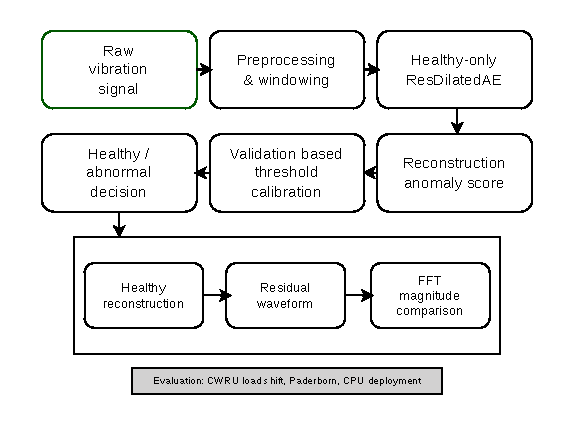
\includegraphics[width=\columnwidth]{diagrams/final_methodology_diagram.pdf}
    \caption{Overview of the final VibeTwin pipeline. A vibration window is reconstructed by a healthy-only ResDilatedAE, scored through reconstruction error, calibrated using held-out healthy data, and interpreted through reconstruction, residual waveform, and FFT-magnitude comparison.}
    \label{fig:methodology}
\end{figure}

\section{Experiment}

\subsection{Experimental Setup}

The final VibeTwin configuration uses the ResDilatedAE backbone with healthy-only training and reconstruction-based anomaly scoring. All experiments use fixed-length vibration windows of length 2048 with stride 1024, and anomaly decisions are obtained by calibrating thresholds on held-out healthy validation data. Evaluation is carried out in two complementary settings. First, CWRU is used with a leakage-safe leave-one-load-out protocol to test operating-condition transfer. Second, Paderborn is used as a cross-benchmark validation setting to assess robustness on a more challenging bearing dataset with multiple operating conditions. In both cases, the goal is not closed-set fault classification, but detection of deviation from learned healthy behavior.

\subsection{Datasets, Protocols, and Baselines}

For CWRU, each fold holds out one motor load for testing. Healthy training and validation windows are drawn only from the remaining loads, while healthy and fault test windows come only from the held-out load. Fold-specific normalization is refit using healthy training windows only, preserving a leakage-safe protocol. This evaluation emphasizes whether a healthy-only reconstruction model can maintain alarm quality when operating conditions shift.

For Paderborn, the model is trained only on healthy bearings and evaluated on healthy and damaged windows across four operating conditions. The processed setup uses the \texttt{vibration\_1} channel with healthy train/validation/test partitions and fault windows reserved for test. In the current pipeline, bearing labels are inferred from bearing-code families, which should be kept in mind when interpreting the results.

VibeTwin is compared against the earlier compact autoencoder baseline and shallow one-class baselines, especially Isolation Forest, which remained the strongest non-neural reference on Paderborn. Performance is reported using AUROC, AUPRC, F1, precision, recall on fault windows, and false-alarm rate.

\subsection{CWRU Load-Shift Results}

\begin{table}[t]
\centering
\caption{CWRU final model versus baseline references under harder leave-one-load-out load shift.}
\label{tab:cwru_results}
\begin{tabular}{p{2.0cm} p{2.2cm} c c c c c}
\toprule
Model & Threshold Setup & AUROC & F1 & Precision & Recall Fault & False Alarm Rate \\
\midrule
AE & saved mean\_plus\_3std & 1.000 $\pm$ 0.000 & 0.984 $\pm$ 0.019 & 0.969 $\pm$ 0.036 & 1.000 $\pm$ 0.000 & 0.301 $\pm$ 0.412 \\
OC-SVM & saved mean\_plus\_3std & 1.000 $\pm$ 0.000 & 0.980 $\pm$ 0.017 & 0.962 $\pm$ 0.032 & 1.000 $\pm$ 0.000 & 0.337 $\pm$ 0.391 \\
Isolation Forest & saved mean\_plus\_3std & 1.000 $\pm$ 0.000 & 0.986 $\pm$ 0.017 & 0.973 $\pm$ 0.033 & 1.000 $\pm$ 0.000 & 0.268 $\pm$ 0.390 \\
ResDilatedAE & saved mean\_plus\_3std & 1.000 $\pm$ 0.000 & 0.987 $\pm$ 0.019 & 0.976 $\pm$ 0.035 & 1.000 $\pm$ 0.000 & 0.257 $\pm$ 0.412 \\
ResDilatedAE & percentile\_99 & 1.000 $\pm$ 0.000 & 0.988 $\pm$ 0.019 & 0.977 $\pm$ 0.036 & 1.000 $\pm$ 0.000 & 0.254 $\pm$ 0.414 \\
\bottomrule
\end{tabular}
\end{table}

Table~\ref{tab:cwru_results} summarizes the harder CWRU leave-one-load-out evaluation. The final ResDilatedAE preserves perfect ranking under load shift, reaching mean AUROC/AUPRC of 1.000/1.000 and mean F1 of 0.987. Relative to the earlier CompactAE, it slightly improves mean F1 and reduces the mean false-alarm rate. It also slightly outperforms the saved Isolation Forest baseline on mean F1 under the same protocol.

However, one held-out load remains problematic. For load 0, the model still ranks faults perfectly, but the false-alarm rate rises sharply, indicating that healthy-score transfer across that condition remains brittle. A follow-up threshold sweep produced only modest overall gains and did not resolve the load-0 false-alarm problem, suggesting that the remaining failure is not mainly caused by the threshold rule alone.

\subsection{Paderborn Results}


Paderborn provides the stronger robustness test for the final generative model. Table~\ref{tab:paderborn_results} and Fig.~\ref{fig:paderborn_threshold} summarize the main findings. A three-seed evaluation of ResDilatedAE shows stable performance, and threshold calibration materially improves the practical operating point. Under the selected \texttt{percentile\_99\_5} rule, the final three-seed mean reaches AUROC 0.858, F1 0.757, recall 0.610, and false-alarm rate 0.007. Compared with the saved Isolation Forest baseline, the calibrated ResDilatedAE improves F1, recall, and false-alarm rate, although Isolation Forest still remains stronger on AUROC.

\begin{table}[t]
\centering
\caption{Paderborn final model versus baseline references. ResDilatedAE results are reported across three seeds.}
\label{tab:paderborn_results}
\begin{tabular}{p{2.2cm} p{2.1cm} c c c c c}
\toprule
Model & Threshold Setup & AUROC & F1 & Precision & Recall Fault & False Alarm Rate \\
\midrule
CompactAE & mean\_plus\_3std & 0.546 & 0.261 & 0.998 & 0.150 & 0.0087 \\
OC-SVM & mean\_plus\_3std & 0.577 & 0.000 & 1.000 & 0.000 & 0.0000 \\
Isolation Forest & mean\_plus\_3std & 0.914 & 0.634 & 0.999 & 0.464 & 0.0083 \\
ResDilatedAE & mean\_plus\_3std & 0.858 $\pm$ 0.013 & 0.770 $\pm$ 0.030 & 0.999 $\pm$ 0.000 & 0.627 $\pm$ 0.040 & 0.0154 $\pm$ 0.0018 \\
ResDilatedAE & percentile\_99\_5 & 0.858 $\pm$ 0.013 & 0.757 $\pm$ 0.022 & 1.000 $\pm$ 0.000 & 0.610 $\pm$ 0.028 & 0.0071 $\pm$ 0.0006 \\
\bottomrule
\end{tabular}
\end{table}

\begin{figure}[t]
    \centering
    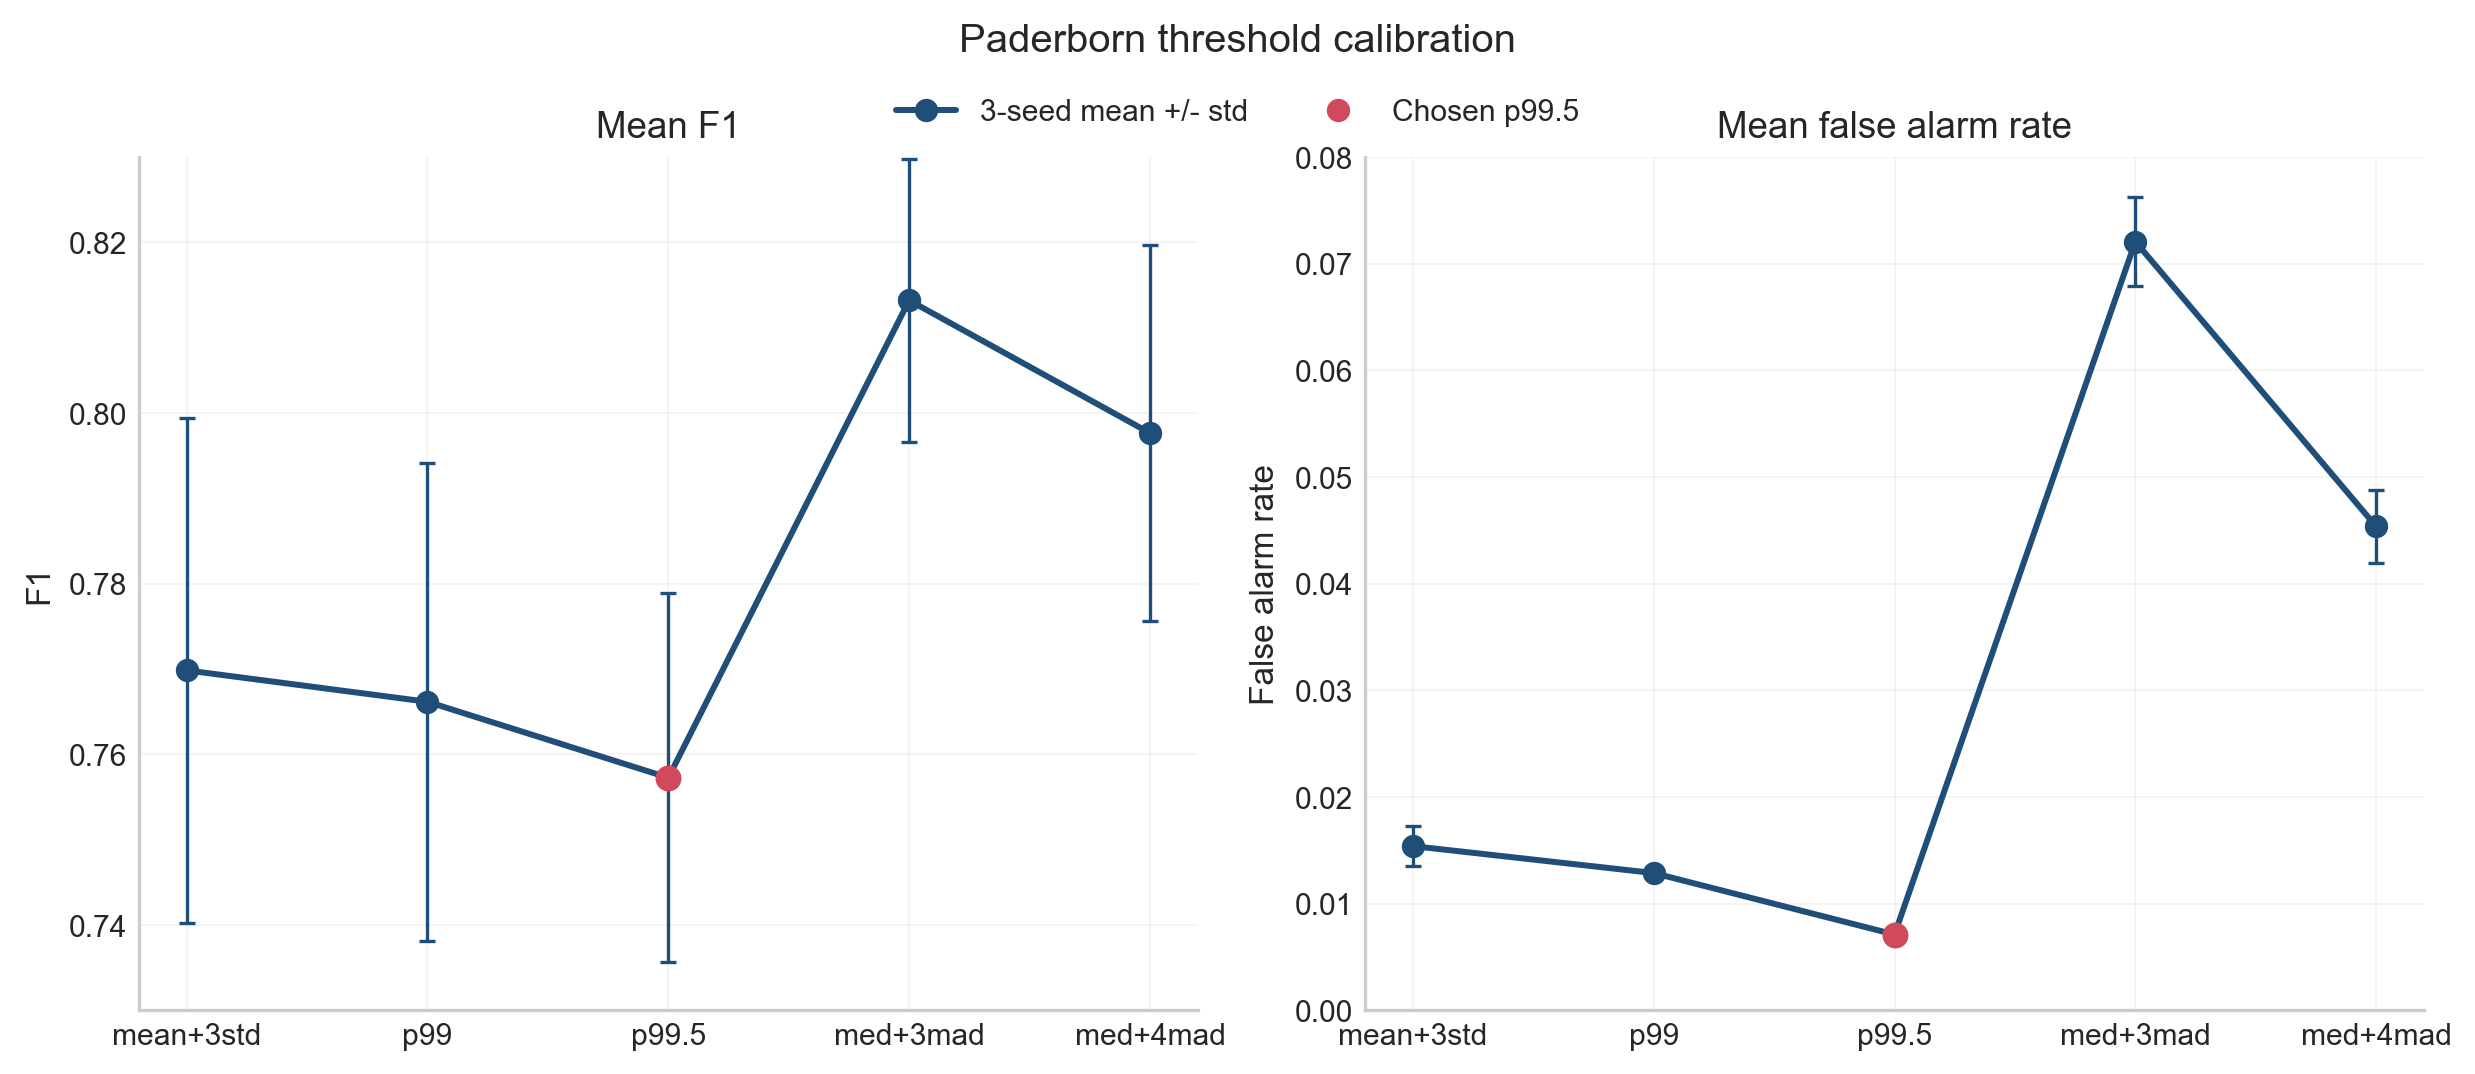
\includegraphics[width=\columnwidth]{figures/paderborn_threshold_calibration_clean.png}
    \caption{Threshold-calibration comparison for ResDilatedAE on Paderborn. The selected \texttt{percentile\_99\_5} rule reduces false alarms substantially while preserving a competitive F1 score.}
    \label{fig:paderborn_threshold}
\end{figure}

These results indicate that strengthening the generative backbone was important: the earlier compact autoencoder performed poorly on Paderborn, while the final residual-dilated model recovers much of the lost performance. At the same time, the remaining AUROC gap to Isolation Forest suggests that ranking and calibration should still be treated separately when evaluating healthy-only monitoring systems.

\subsection{Explanation and Deployment Proof of Concept}

To support interpretability, VibeTwin generates qualitative explanation case studies using the final calibrated Paderborn model. Figure~\ref{fig:explanation_case} illustrates a representative abnormal window through the original signal, its healthy reconstruction, the residual waveform, and FFT-magnitude comparison. These views provide a direct qualitative explanation of why a window is considered close to or far from the learned healthy reference.

Deployment-oriented profiling was also performed on CPU. The final ResDilatedAE contains 222,657 parameters, occupies approximately 0.88 MB on disk, and runs in about 8.8 ms per window on CPU. Although this is materially heavier than the earlier compact autoencoder, it remains practical for industrial-PC or gateway-style deployment while offering a large improvement in monitoring quality.

\begin{figure}[t]
    \centering
    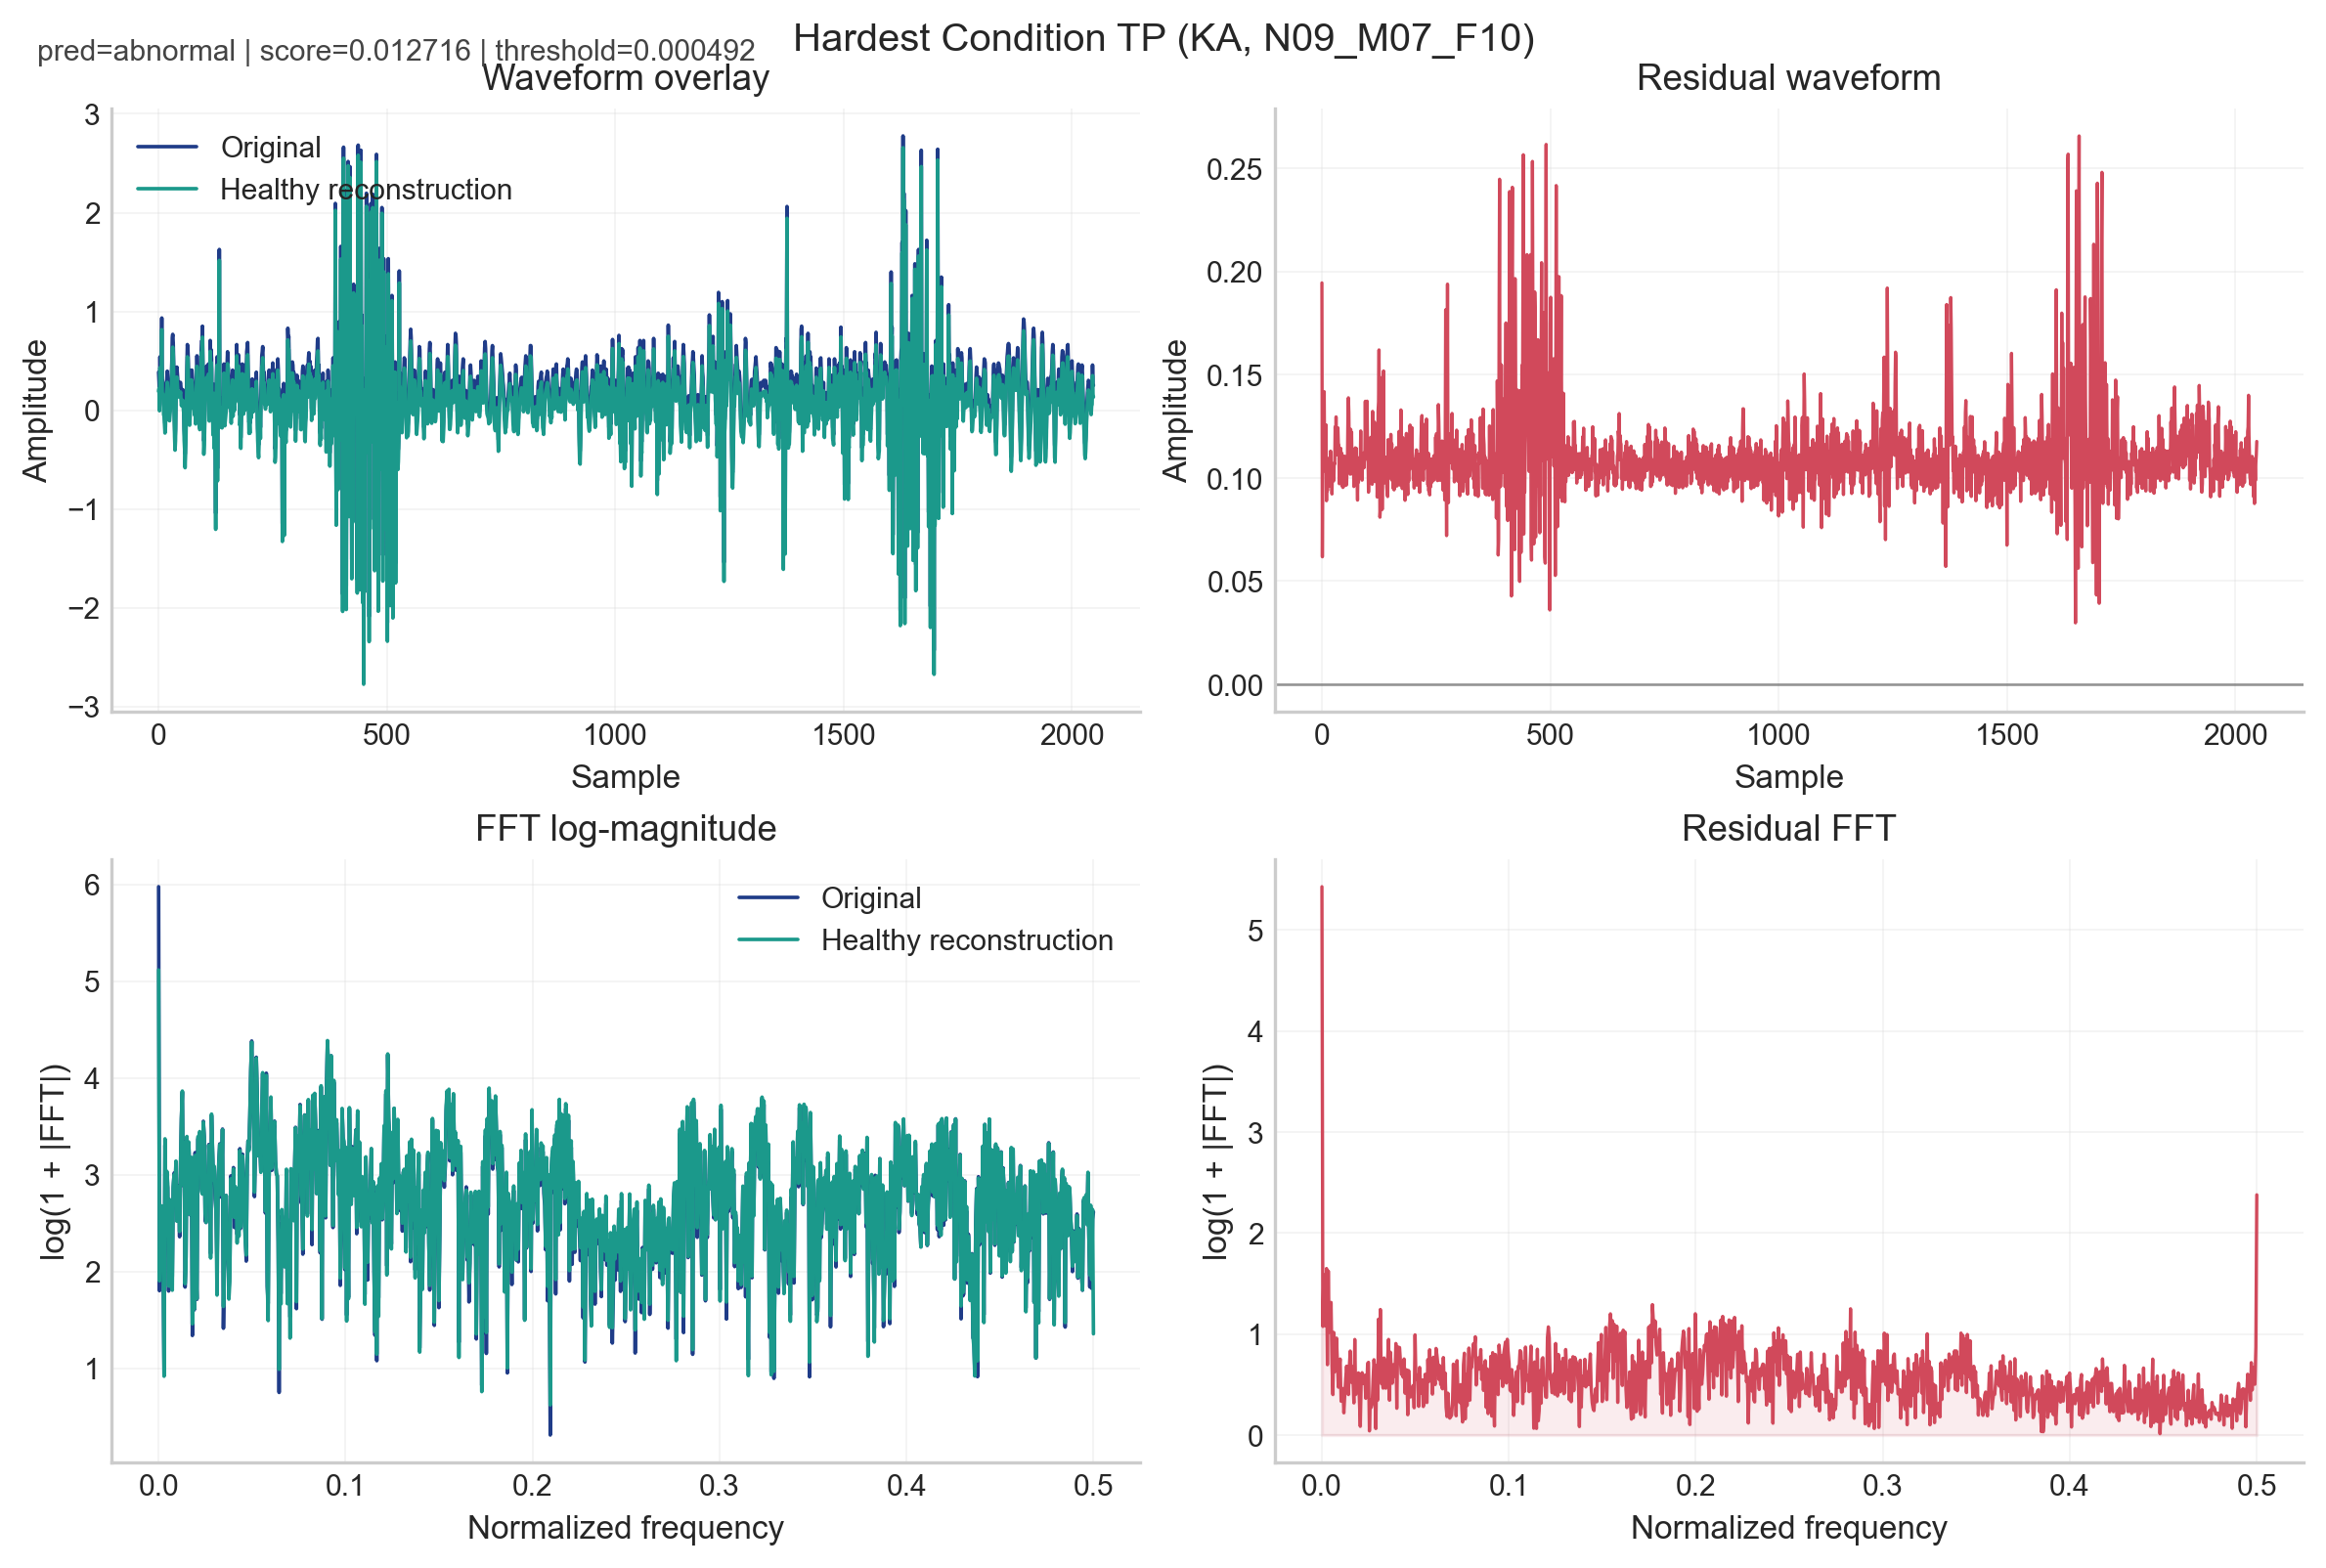
\includegraphics[width=\columnwidth]{figures/explanation_hardest_condition_clean.png}
    \caption{Representative explanation case from the hardest Paderborn operating condition. The figure shows the original vibration window, its healthy reconstruction, the residual waveform, and FFT-magnitude comparison.}
    \label{fig:explanation_case}
\end{figure}

\section{Discussion}

The experiments suggest that the main strength of VibeTwin is not simply the use of reconstruction error, but the combination of a stronger healthy-only generative backbone with explicit threshold calibration. On CWRU, the final ResDilatedAE preserves perfect ranking under the harder leave-one-load-out protocol and slightly improves over the earlier compact autoencoder and saved shallow baselines in mean F1 and false-alarm rate. This indicates that the model learns a strong representation of healthy versus abnormal behavior even when operating conditions shift. However, the held-out load-0 fold remains a clear failure case: faults are still ranked correctly, but healthy windows from that condition are frequently flagged as abnormal. The follow-up threshold sweep produced only marginal gains and did not resolve this behavior, suggesting that the remaining weakness is not mainly due to a poor threshold rule, but to a deeper mismatch in how healthy patterns transfer across operating conditions.

Paderborn presents a different and more realistic challenge. Here, the earlier compact autoencoder was clearly too weak, while the final ResDilatedAE recovered much stronger performance, especially after calibration. The calibrated three-seed results show that the generative approach can become practically competitive: compared with the saved Isolation Forest baseline, the final system improves F1, recall, and false-alarm rate, although Isolation Forest still remains stronger on AUROC. This distinction is important. It means the shallow baseline still provides slightly better overall ranking, but the calibrated generative model offers a more favorable operating point for fault monitoring, especially when recall and alarm quality matter more than rank alone. In that sense, the final paper story is not that generative modeling universally dominates shallow baselines, but that a stronger reconstruction model plus calibration can produce a useful and credible healthy-only monitoring system.

The additional studies also clarify what should and should not be claimed. The qualitative explanation module is a useful proof of concept: healthy reconstruction, residual waveform inspection, and FFT-based comparison provide an interpretable view of why a window was judged close to or far from the learned healthy reference. At the same time, these explanations should be presented as qualitative case studies rather than as formally validated explanation metrics. Similarly, the MC-dropout study is valuable mainly as a negative result. Although uncertainty-based deferral reduced false alarms, it did so by deferring too many windows and sharply degrading F1 and recall, so uncertainty estimation was not retained as part of the final operating pipeline. This is still informative, because it shows that uncertainty estimation cannot be assumed to improve practical reliability without careful validation.

Finally, the deployment results help place the method in a realistic application context. The final model remains compact on disk and fast enough for CPU inference, supporting an industrial-PC or gateway-style deployment story. It is not, however, a microcontroller-class solution, and the runtime memory increase should be acknowledged clearly. More broadly, the current study still has limitations that matter for interpretation. Paderborn labels are inferred from bearing-code families rather than fully verified through parsed documentation, and the saved Paderborn Isolation Forest pipeline does not include a serialized model artifact for a perfectly matched deployment benchmark. Taken together, these results support a balanced conclusion: VibeTwin demonstrates that calibrated healthy-only generative monitoring can be practical and interpretable, but robust threshold transfer under condition shift remains an open challenge rather than a solved problem.

\bibliographystyle{ieeetr}
\bibliography{vibetwin_refs}

\end{document}